\chapter{Análisis estadístico}

%Teniendo los datos guardados y limpios, proseguimos con la siguiente etapa del proyecto, se realizó un análisis estadístico de los datos. Para ello se observaron los grupos de datos en los que se dividió la información, se eligió el método Holt-Winters aditivo el cual funciona para series de tiempo con componentes de tendencia aproximadamente lineal y de estacionalidad.

%Teniendo los datos guardados y limpios, se realizó un análisis estadístico de los datos, las herramientas elegidas para dicho análisis fueron las series de tiempo y el método Holt-Winters aditivo el cual funciona para series de tiempo con componentes de tendencia aproximadamente lineal y de estacionalidad.


Debido a que los datos obtenidos no son independientes entre sí, las herramientas elegidas para realizar un análisis estadístico de los datos fueron las series de tiempo. A continuación se describe su definición y aplicación para explicar el motivo de la elección de dichas herramientas estadísticas.

Definimos a una serie de tiempo como una secuencia de observaciones $X_{t}$ ordenadas cronológicamente, en donde los datos al tiempo presente dependen de las observaciones anteriores, es decir existe una depencia de $X_{t}$ con $\{X_{t-1}, X_{t-2}, X_{t-3}, \ldots, X_{1}\}$.

Denotamos a una serie de tiempo como:
\begin{equation}
X_{t} = m_{t} + s_{t} + y_{t}
\end{equation}
%Se dice que una serie de tiempo es estacionaria si a lo largo del tiempo su media y su varianza con constantes y es no estacionaria si su tendencia y variabilidad cambian en el tiempo. Sus componentes son:
Cada elemento de la serie de tiempo es llamado componente. A continuación se describe cada una de ellas.

\begin{itemize}
\item[-] Tendencia $(m_{t})$: Se le llama tendencia al cambio a largo plazo del promedio de los datos. El cambio puede ser creciente o decreciente.

\item[-] Estacionalidad $(s_{t})$: Se llama variación estacional a las fluctuaciones periódicas que tiene una serie de tiempo. La longitud de cada periodo es constante y menor o igual a un año, por ejemplo semanal, mensual o semestral.

\item[-] Aleatoriedad $(y_{t})$: También llamada componente irregular, son series de residuales que pueden o no ser aleatorios.
\end{itemize}

Chatfield y Xing nos indican, en su libro \textit{The Analysis of Time Series An Introduction with R} (\ref{ChatfieldXing}), que existen 2 tipos de variación estacional:

\begin{itemize}
\item[-] Aditiva: Se dice que la estacionalidad es aditiva cuando la longitud de cada periodo es constante año con año.

\item[-] Multiplicativa: Se dice que la estacionalidad es multiplicativa cuando la longitud de cada periodo es directamente proporcional a la media de los datos de la serie de tiempo.
\end{itemize}

Con estos tipos de variaciones se forman 3 modelos de estacionalidad:

\begin{enumerate}
\item Aditivo: Se tiene variación estacional aditiva y se utiliza cuando la varianza o la desviación estándar de la serie de tiempo se mantienen constantes a lo largo del tiempo.
\begin{equation}
X_{t} = m_{t} + s_{t} + y_{t}
\end{equation}

\item Multiplicativo: Se tiene variación estacional multiplicativa. Se utiliza cuando la varianza o la desviación estándar de los datos cambian a través del tiempo. Su variabilididad puede ser mayor o menor conforme pasa el tiempo.
\begin{equation}
X_{t} = m_{t}s_{t}y_{t}
\end{equation}

\item Mixto: Se utiliza cuando se tiene variación estacional multiplicativa pero la variabilidad de la componente irregular se mantiene constante a lo largo del tiempo.
\begin{equation}
X_{t} = m_{t}s_{t} + y_{t}
\end{equation}
\end{enumerate}

Los objetivos principales al hacer el análisis de una serie de tiempo son:

\begin{itemize}
\item[-] Describir: Leer datos en una tabla es mucho más tardado y en algunas ocasiones más complicado que observar una gráfica de los datos que se tienen. Las gráficas ayudan a ver de una manera más inmediata el comportamiento que tienen los datos y es posible observar si la serie de tiempo tiene alguna tendencia o estacionalidad. También se puede ver la posible falta de información o valores atípicos.

\item[-] Predecir: Teniendo una serie de tiempo se desea conocer qué va a pasar en el futuro. Es conveniente tener varios periodos de información para que la predicción sea lo más acertada posible.
\end{itemize}

Las áreas en las que se pueden aplicar las series de tiempo son por ejemplo en economía, demografía, finanzas, medio ambiente, ingeniería o medicina. Algunos ejemplos más precisos de su aplicación son: precios de acciones diarios, niveles de producción en la agricultura mensuales, medición del sonido por segundos, electrocardigramas, medición de terremotos, tasa de mortalidad, tasa de natalidad, barriles de petróleo producidos al año, entre otros.


\section{Análisis estadístico básico}

En esta sección se hará un análisis de los datos obtenidos. Las técnicas de suavizamiento de series de tiempo son útiles para mostrar patrones subyacentes en los datos de las series de tiempo. El método que se va a utilizar para mostrar dichos patrones y para realizar predicciones de los datos es el método Holt-Winters aditivo.

%El método Holt-Winters aditivo se utiliza para describir y predecir valores con series de tiempo que tienen componentes de tendencia aproximadamente lineal y de estacionalidad.

El método se utiliza para describir y predecir valores con series de tiempo que tienen componentes de tendencia y de estacionalidad. Existen pruebas, que hemos hecho a los datos, para comprobar que los datos que obtuvimos cumplen con los supuestos del método. Éstas pruebas se muestran a lo largo de esta sección.

Primero se van a graficar los datos como serie de tiempo y después se van a mostrar algunas gráficas de barras. Vamos a observar el comportamiento de los datos, ver si tiene alguna tendencia y variación estacional.

%En la siguiente figura se muestra la gráfica con el número total de alumnos que toman clases por semestre. A simple vista notamos que tiene una tendencia creciente y una estacionalidad semestral. Podemos ver también que 
%\begin{figure}[H]
%\centering
%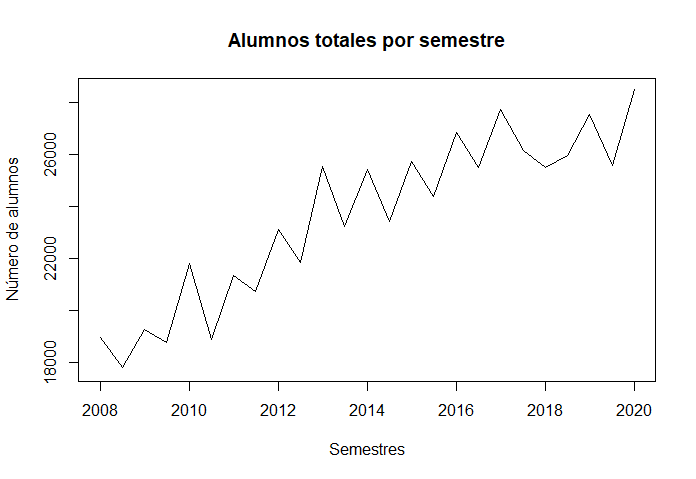
\includegraphics[scale = 0.8]{num_alum_total_x_sem_ts} %width=\textwidth
%\caption{\textit{Número total de alumnos por semestre: Serie de tiempo}}
%\end{figure}

En la figura \ref{TotalAlumBarras} se muestra la gráfica de barras con el número total de alumnos que toman clases por semestre. A simple vista notamos que tiene una tendencia creciente y una estacionalidad semestral. Podemos ver también que el número de alumnos de los semestres impares es siempre mayor al de los semestres pares. Éste fenómeno los vimos en la figura \ref{ParImparProbaI} al hacer el análisis correspondiente a los datos de la materia de Probabilidad I.

\begin{figure}[H]
\centering
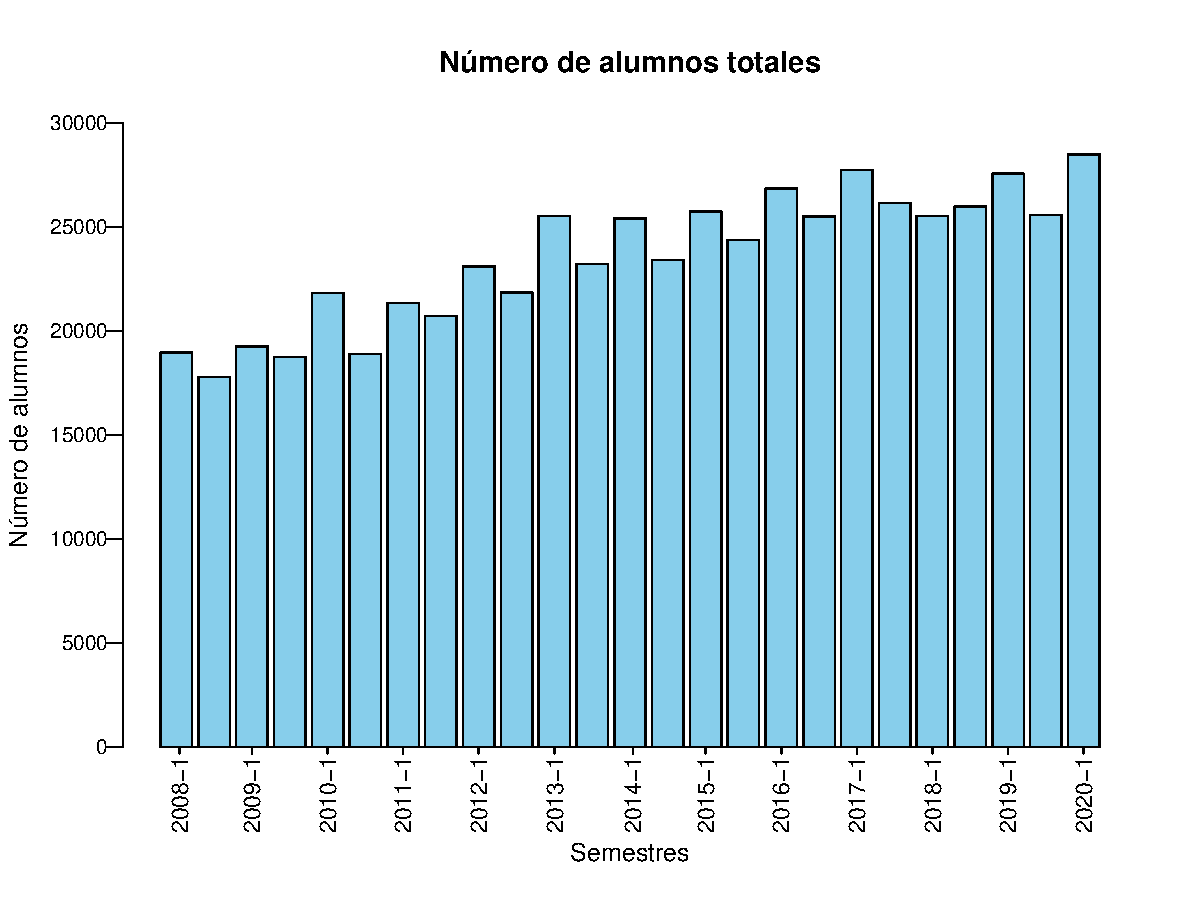
\includegraphics[scale = 0.8]{num_alum_total_x_sem_barplot} %width=\textwidth
\caption{\textit{Número total de alumnos por semestre}}\label{TotalAlumBarras}
\end{figure}

En la figura \ref{prom_alum_x_sem_ts} se muestra la gráfica de la media del número de alumnos que toman clases por semestre de todas las materias. Observamos que los valores tienen una tendencia creciente, esto nos indica que cada semestre, en promedio hay más alumnos tomando clases en la FC.

\begin{figure}[H]
\centering
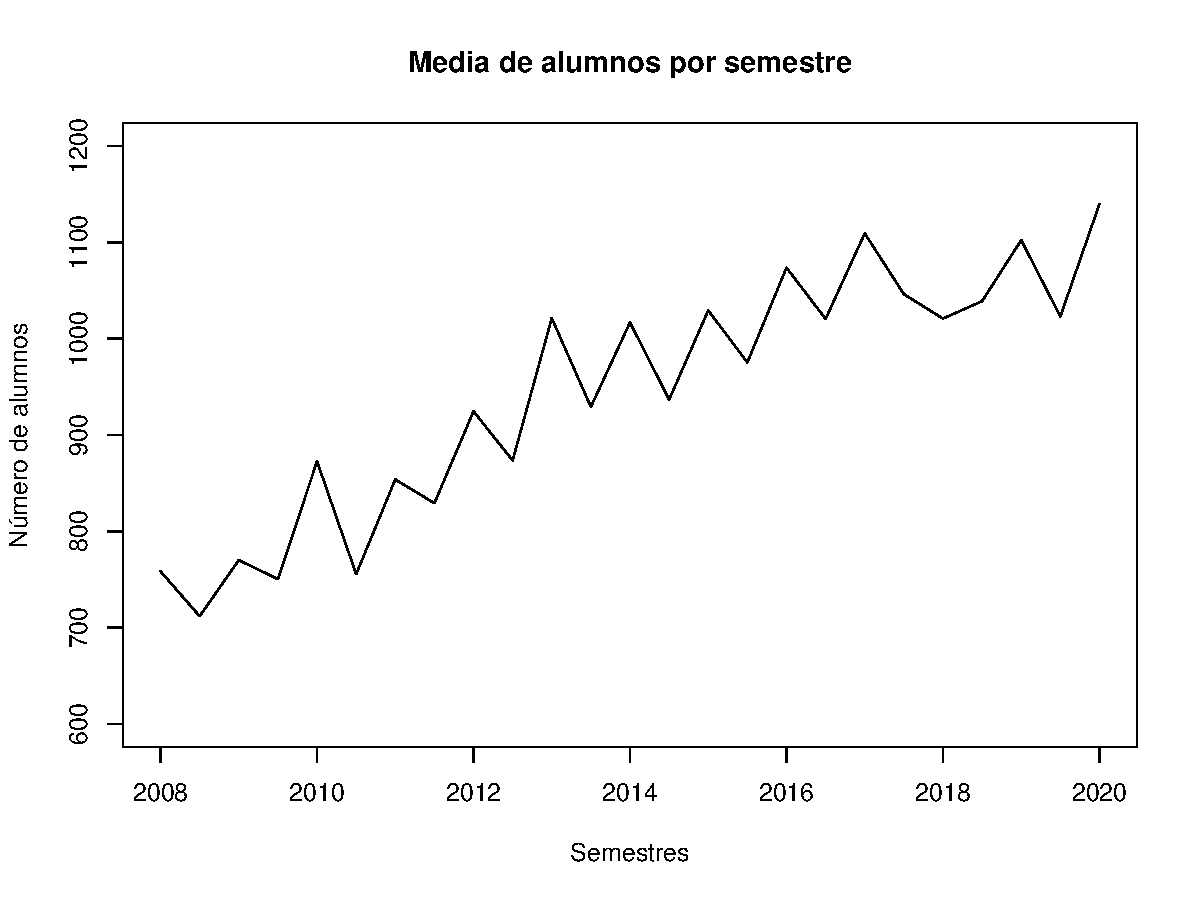
\includegraphics[scale = 0.8]{prom_alum_total_x_sem_ts.pdf} %width=\textwidth
\caption[\textit{Media de alumnos por semestre}]{\textit{Media de alumnos por semestre: Se observa una tendencia creciente}}\label{prom_alum_x_sem_ts}
\end{figure}

En la figura \ref{sd_alum_x_gpo_x_sem_ts} se muestra la gráfica de la desviación estándar del número de alumnos por grupo y por semestre de todas las materias. Observamos que los valores se mantienen constantes a lo largo del tiempo. Su rango se encuentra entre 24 y 29.

\begin{figure}[H]
\centering
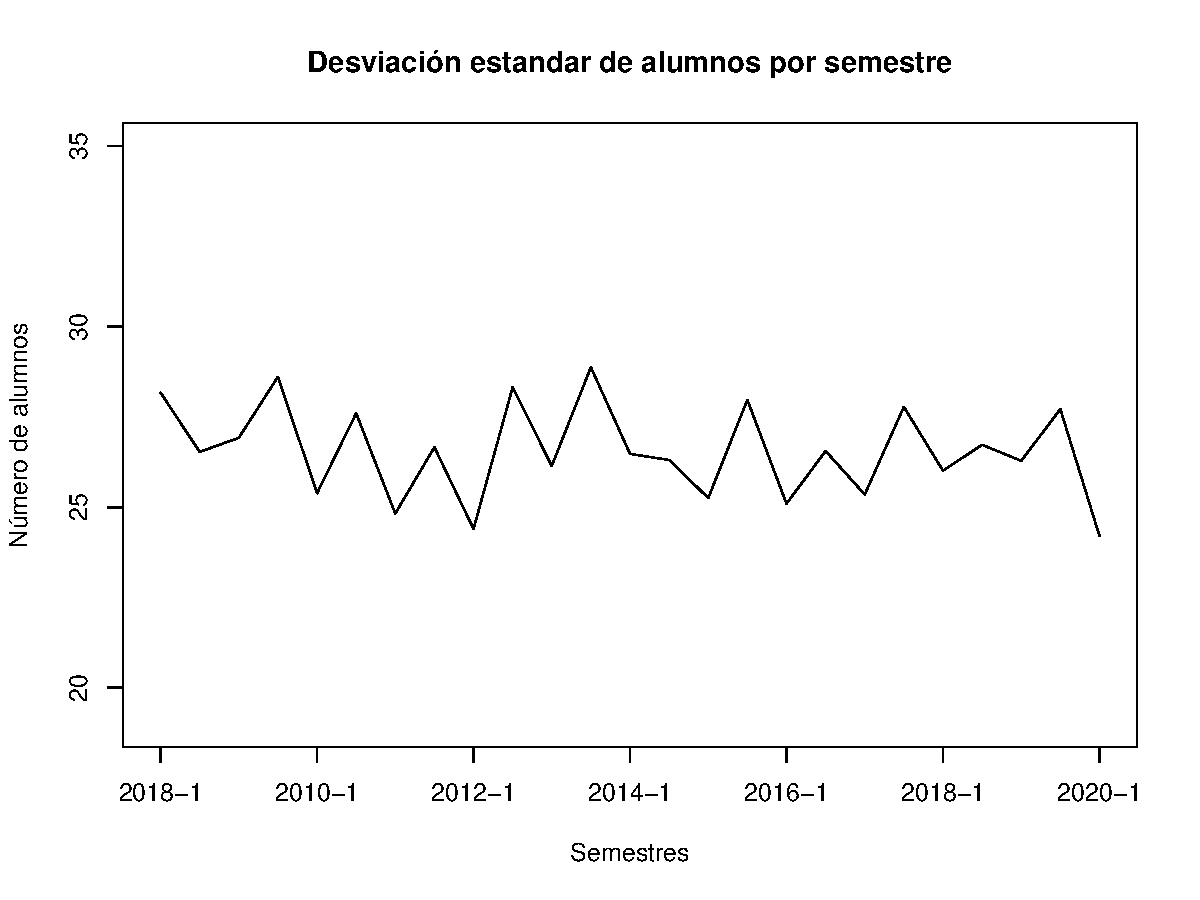
\includegraphics[scale = 0.8]{sd_alum_x_gpo_x_sem_ts.pdf} %width=\textwidth
\caption{\textit{Desviación estándar del número de alumnos por semestre}}\label{sd_alum_x_gpo_x_sem_ts}
\end{figure}

En la figura \ref{img_en_ing_2} se observan 4 diferentes gráficas, en la primera se observan los datos reales. En la segunda la tendecia de los datos, la cual notamos que es creciente. En la tercera la componente estacional que nos indica que los datos tienen una estacionalidad semestral. En la cuarta se ve la componente aleatoria de los datos la cual ya no tiene estacionalidad ni tendencia.

\begin{figure}[H]
\centering
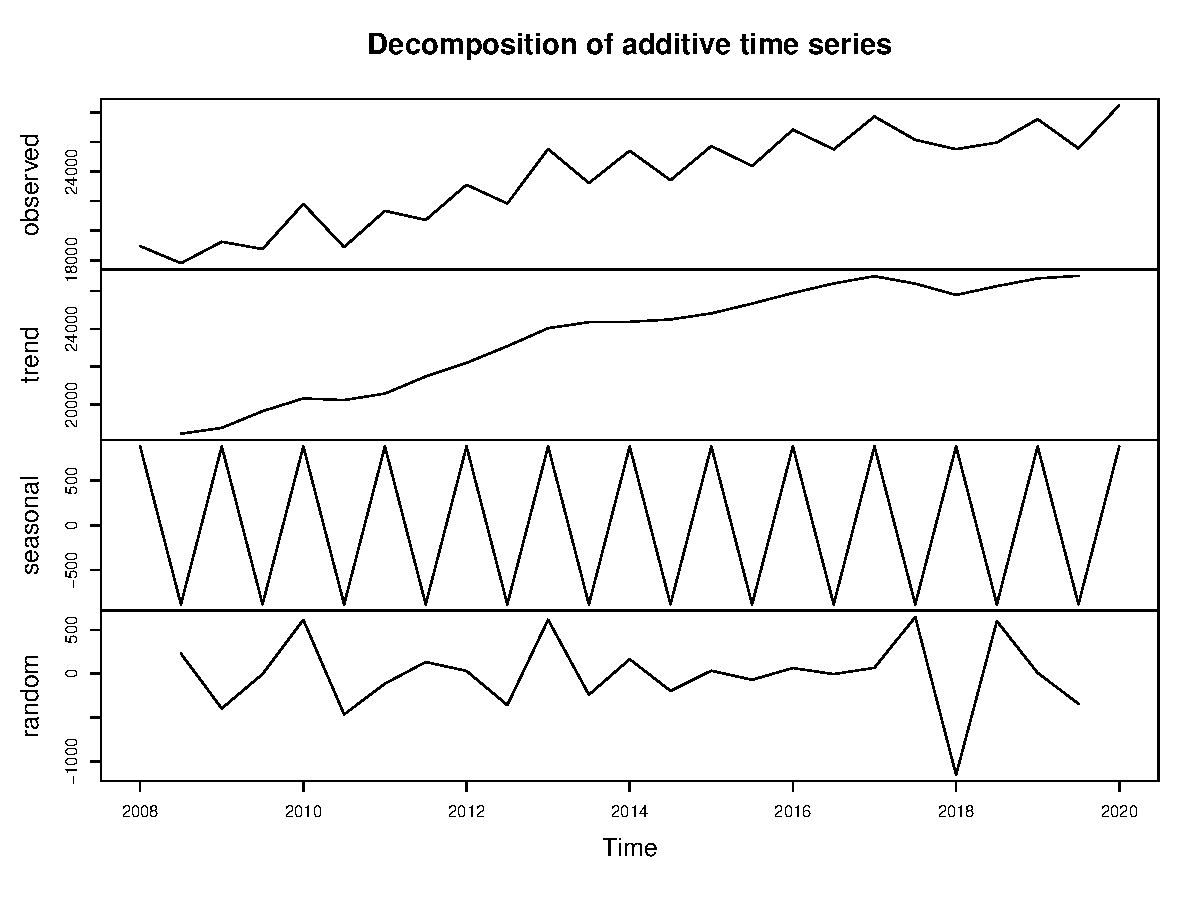
\includegraphics[scale = 0.8]{descomposicion_ts_total_alumnos.pdf} %width=\textwidth
\caption{\textit{Descomposición por el método aditivo de Holt-Winters: Total de alumnos por semestre}}\label{img_en_ing_2}
\end{figure}

Observando la figura \ref{img_en_ing_2} notamos que los datos tienen estacionalidad semestral y una tendencia creciente, por lo tanto confirmamos que se puede utilizar el método Holt-Winters ya que se cumplen los supuestos que se requieren. Para verificar que el modelo de estacionalidad adecuado es el aditivo, vemos la figura \ref{sd_alum_x_gpo_x_sem_ts} y notamos que la desviación estándar permanece constante a lo largo del tiempo.


\section{Análisis estadístico por grupo de datos} \label{AE_x_GpoDeDatos}

En la figura \ref{NumAlTotal_ParImpar_ts} se muestra la gráfica del número de alumnos separado por semestres pares e impares. Se observa un comportamiento similar al de la figura \ref{ParImparProbaI}. Vemos con mayor claridad lo que ocurre en la figura \ref{TotalAlumBarras}, los datos efectivamente tienen una tendencia creciente. Sin embargo notamos que el número de alumnos de los semestres impares es mayor al número total de alumnos de los semestres pares, salvo en el semestre 2018-1 en donde el número de alumnos es menor a los de los semestres adyacentes, los cuales son el 2017-2 y el 2018-2.

\begin{figure}[H]
\centering
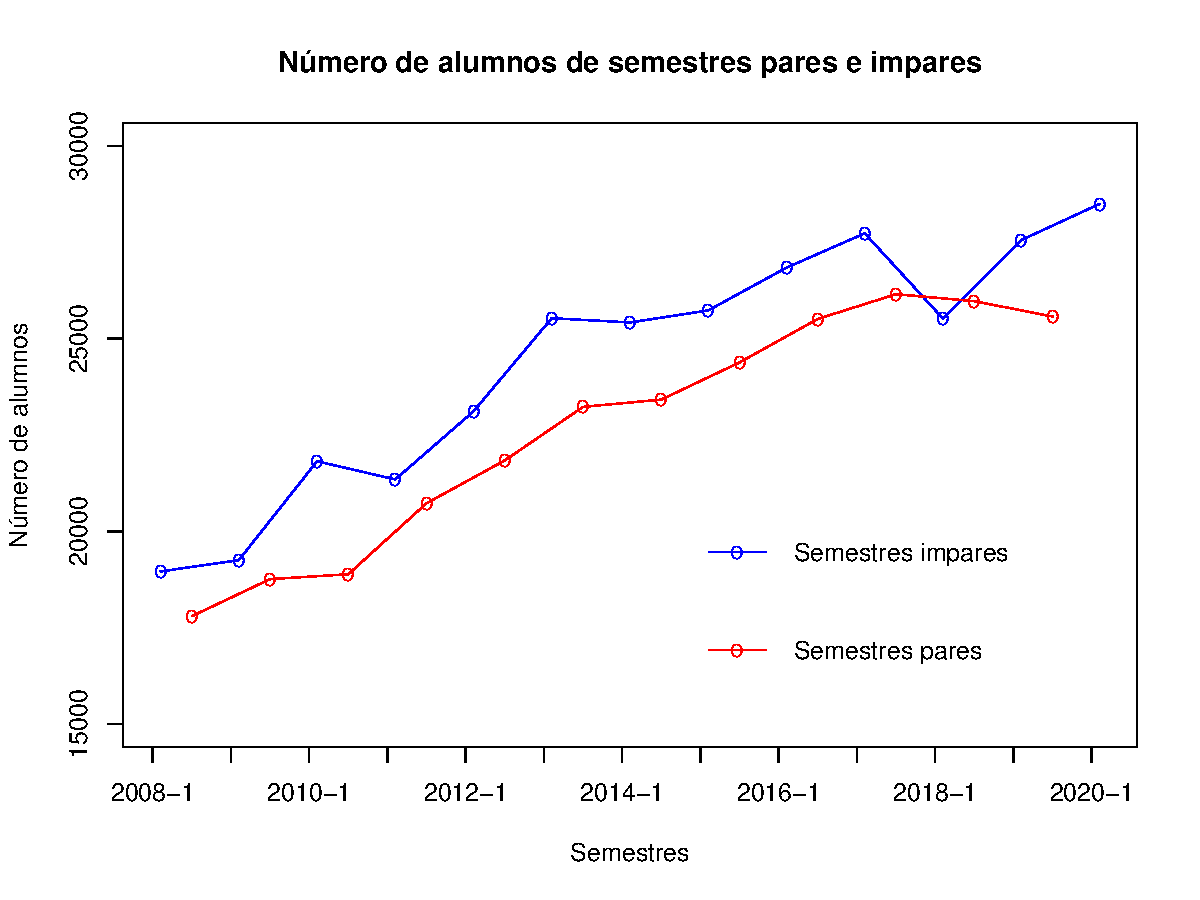
\includegraphics[scale = 0.8]{num_alum_sem_par_impar_ts.pdf} %width=\textwidth
\caption{\textit{Número de alumnos de semestres pares e impares}}\label{NumAlTotal_ParImpar_ts}
\end{figure}


En la figura \ref{histNumAlTotal_ParImpar} se muestra el histograma doble del número total de alumnos de semestres pares e impares con sus respectivas densidades ajustadas. Notamos que hay una ligera diferencia entre el número de alumnos de los semestres pares con respecto al número de alumnos de los semestres impares. Existe una mayor cantidad de grupos en los semestres pares con un menor número de alumnos. Hay una mayor cantidad de grupos en los semestres impares contra los semestres pares, que tienen entre 35 y 100 alumnos.

Tanto para los semestres pares como para los impares, el comportamiento de la distribución que mejor se le ajusta a los datos es la Poisson, así como lo vimos en la figura \ref{histNumAl_x_gpo_x_sem}.

\begin{figure}[H]
\centering
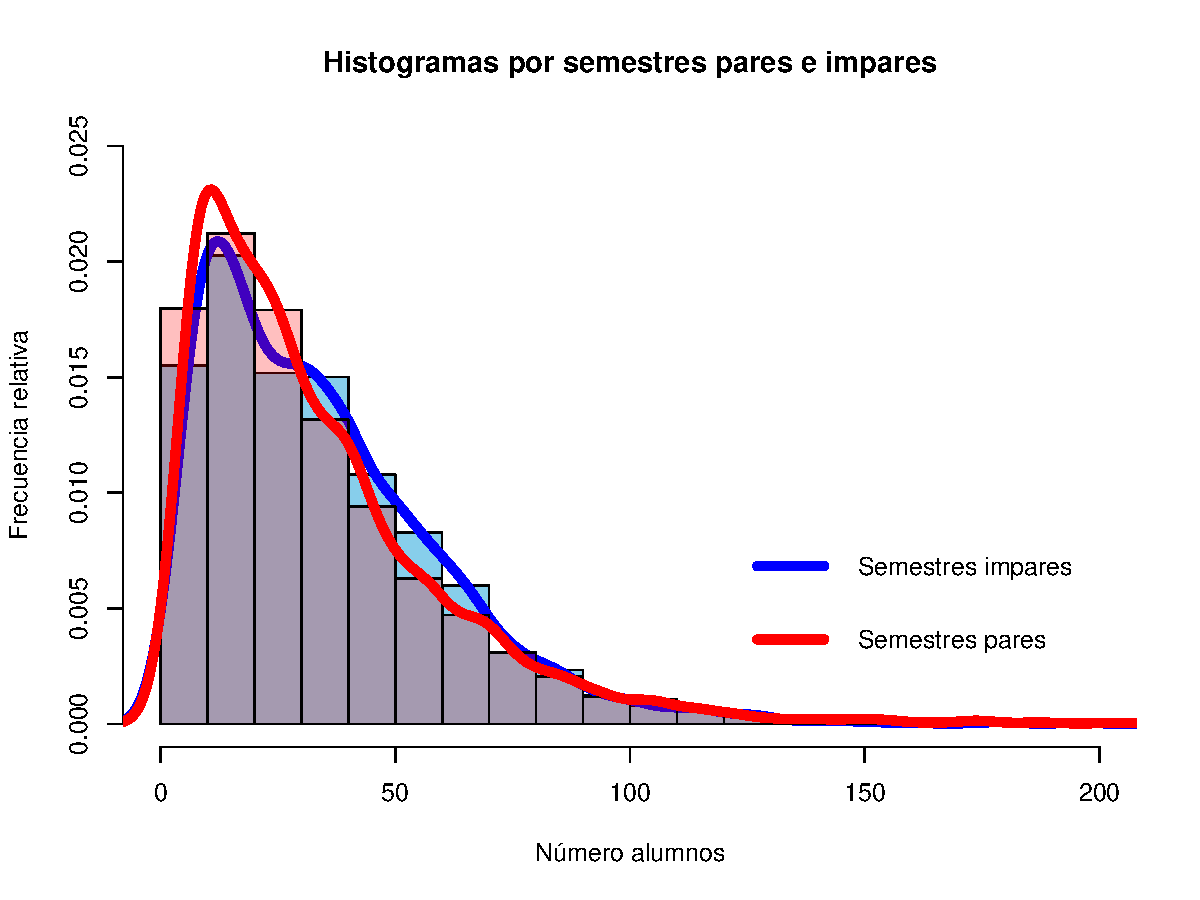
\includegraphics[scale = 0.8]{histograma_FR_num_alum_sem_par_impar.pdf} %width=\textwidth
\caption{\textit{Histograma del número de alumnos de semestres pares e impares}}\label{histNumAlTotal_ParImpar}
\end{figure}


En la figura \ref{NumAlTotal_MatuVesp_ts} se muestra la gráfica del número de alumnos por turno: matutino y vespertino. Se puede observar que en todo momento el número de alumnos del turno matutino es mayor al número de alumnos del turno vespertino. Este comportamiento lo observamos en la figura \ref{num_alum_x_turno_Proba_I} al hacer el anáilisis para la materia de \textit{Probabilidad I}.

\begin{figure}[H]
\centering
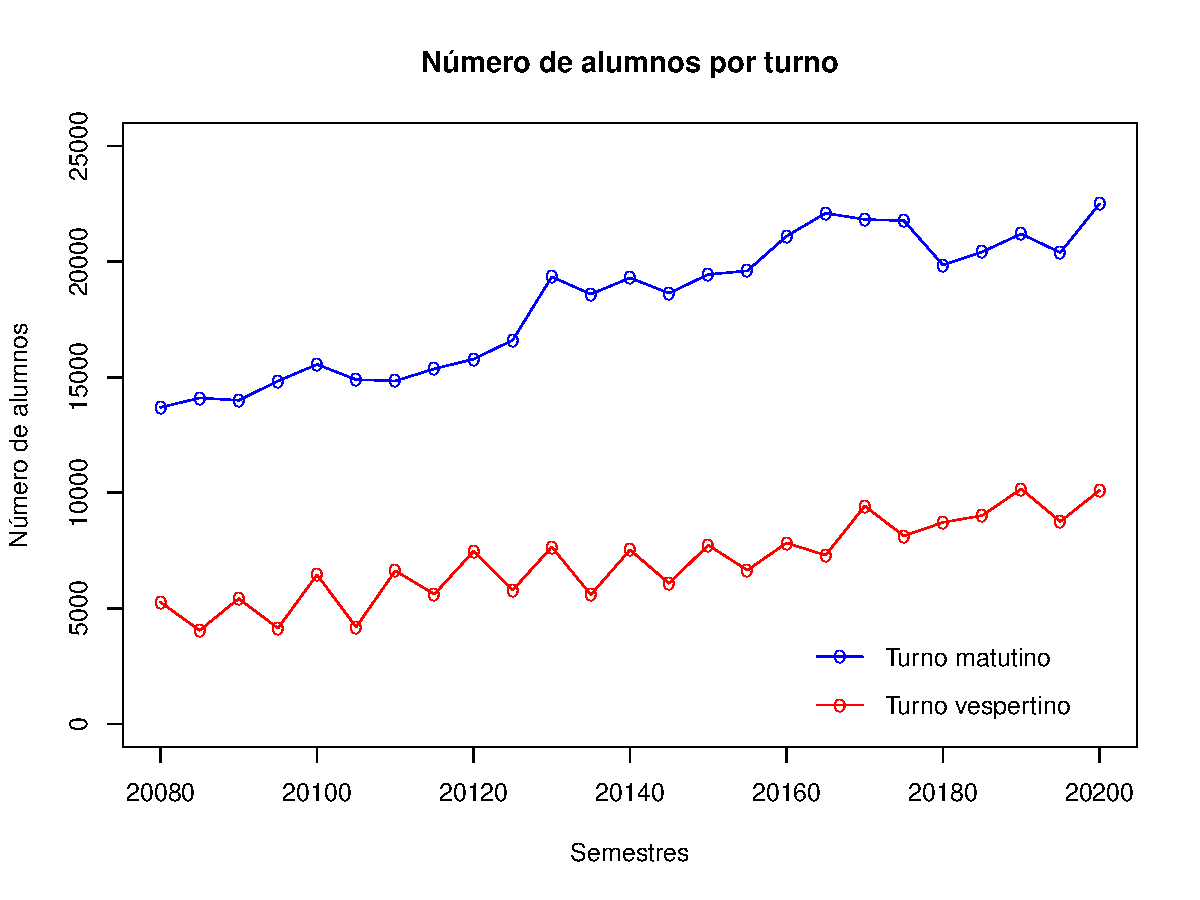
\includegraphics[scale = 0.8]{num_alum_matu_vesp_ts.pdf} %width=\textwidth
\caption{\textit{Número de alumnos por turno de todos los semestres}}\label{NumAlTotal_MatuVesp_ts}
\end{figure}



Los datos que se graficaron en el histograma de la figura \ref{histNumAlTotal_MatuVesp} son los alumnos totales por hora de cada semestre. En dicha figura se muestra el histograma doble de los datos divididos en los turnos matutino y vespertino. Notamos que la diferencia entre cada turno es evidente. Al ver la gráfica podemos concluir que hay más alumnos en el turno matutino que en el vespertino.

\begin{figure}[H]
\centering
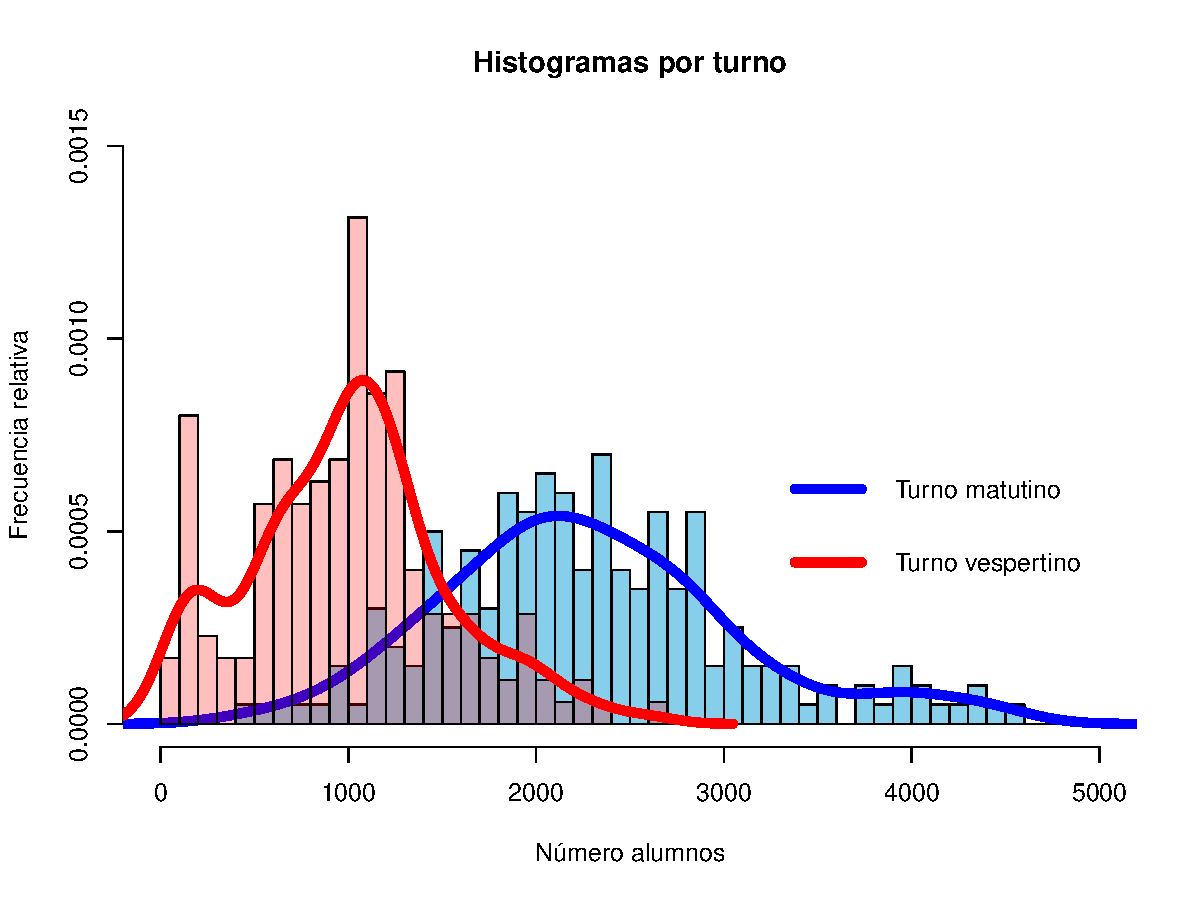
\includegraphics[scale = 0.8]{histograma_FR_num_alum_matu_vesp.pdf} %width=\textwidth
\caption{\textit{Histograma del número de alumnos de los turnos matutino y vespertino}}\label{histNumAlTotal_MatuVesp}
\end{figure}


\section{Análisis estadístico por carrera}

En la figura \ref{histFAnumAl_x_carrera} vemos un histograma para cada carrera con el número de alumnos por grupos. Máximo CdC 211, máx de otras 353.

\begin{figure}[H]
\centering
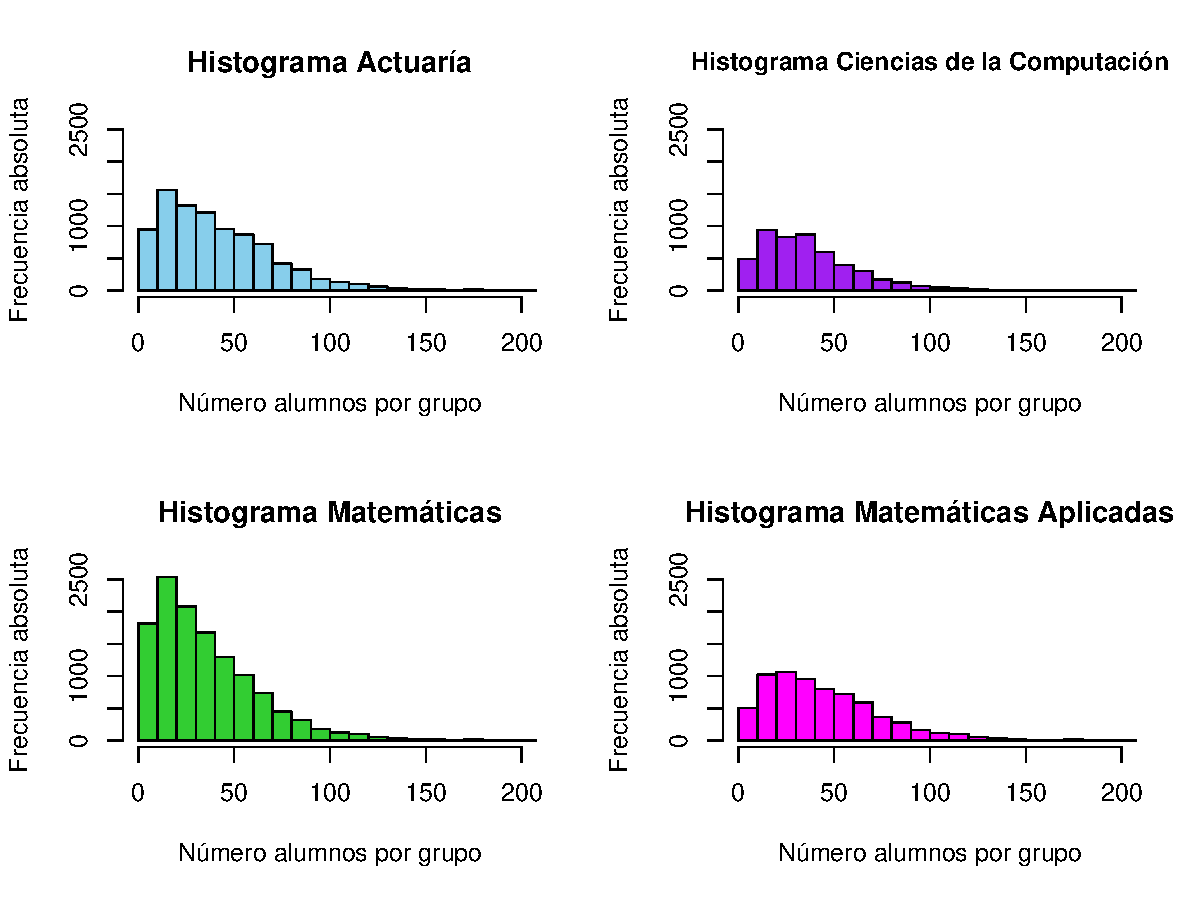
\includegraphics[scale = 0.8]{histogramas_FA_num_alum_x_carrera.pdf} %width=\textwidth
\caption{\textit{Histograma del número de alumnos por carrera}}\label{histFAnumAl_x_carrera}
\end{figure}


En la figura \ref{histFRnumAl_x_carrera} vemos una gráfica con las densidades ajustadas a los datos del número de alumnos por grupos para cada carrera.

\begin{figure}[H]
\centering
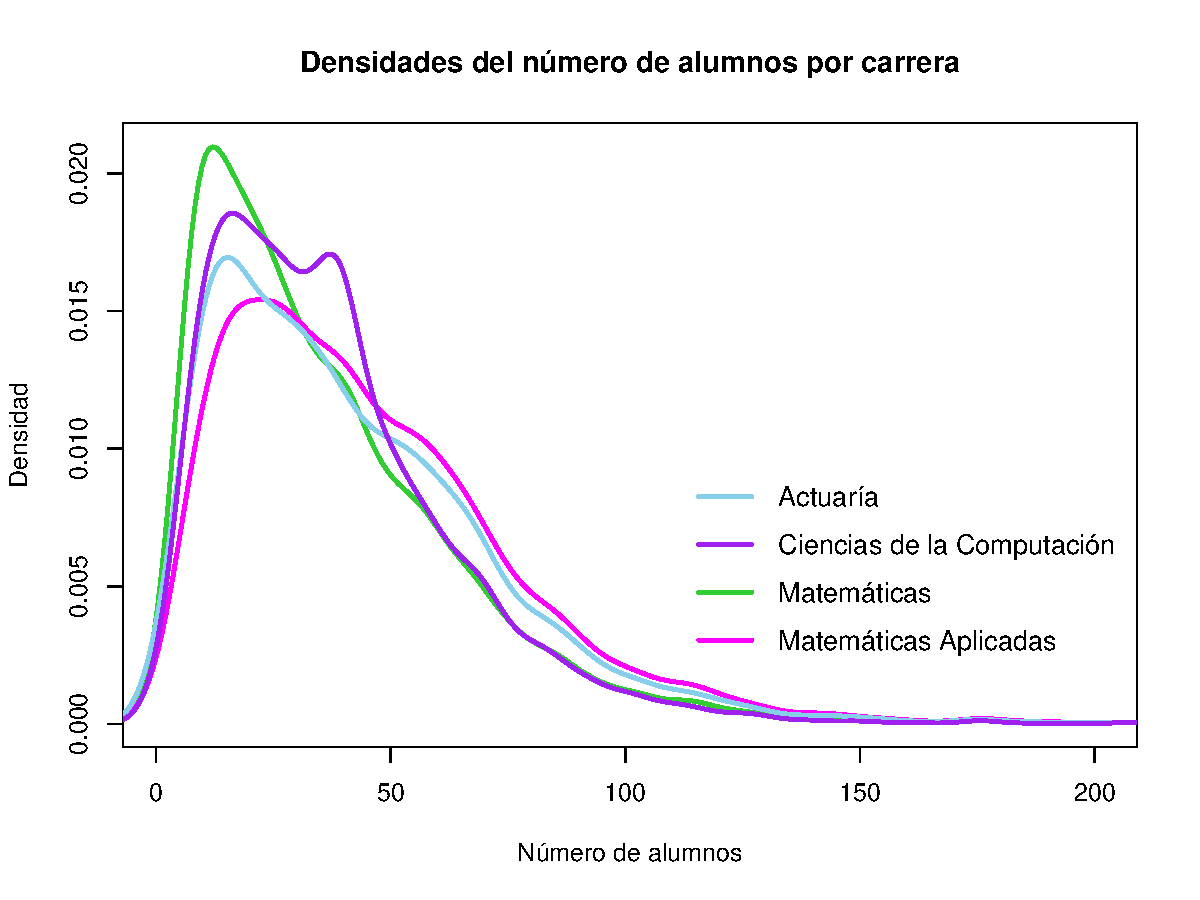
\includegraphics[scale = 0.8]{histogramas_FR_num_alum_x_carrera.pdf} %width=\textwidth
\caption{\textit{Densidades del número de alumnos por carrera}}\label{histFRnumAl_x_carrera}
\end{figure}


%\section{Distribución del número de alumnos por grupo / tamaño de grupo}
\section{Distribución del tamaño de los grupos} \label{DitribTamGpos}
%En la figura \ref{histNumAl_x_gpo_x_sem} se muestra el histograma del número de alumnos por grupo de todos los semestres. En la gráfica de la izquierda se tienen todos los datos. En la gráfica de la derecha se quitó el valor de un grupo con 353 alumnos. Con estas gráficas podemos concluir que la distribución que se ajusta al tamaño de los grupos es una distribución Poisson.
En la figura \ref{histNumAl_x_gpo_x_sem} se muestra el histograma del número de alumnos por grupo de todos los semestres. %La distribución que mejor se ajusta a estos datos es la distribución Poisson.

\begin{figure}[H]
\centering
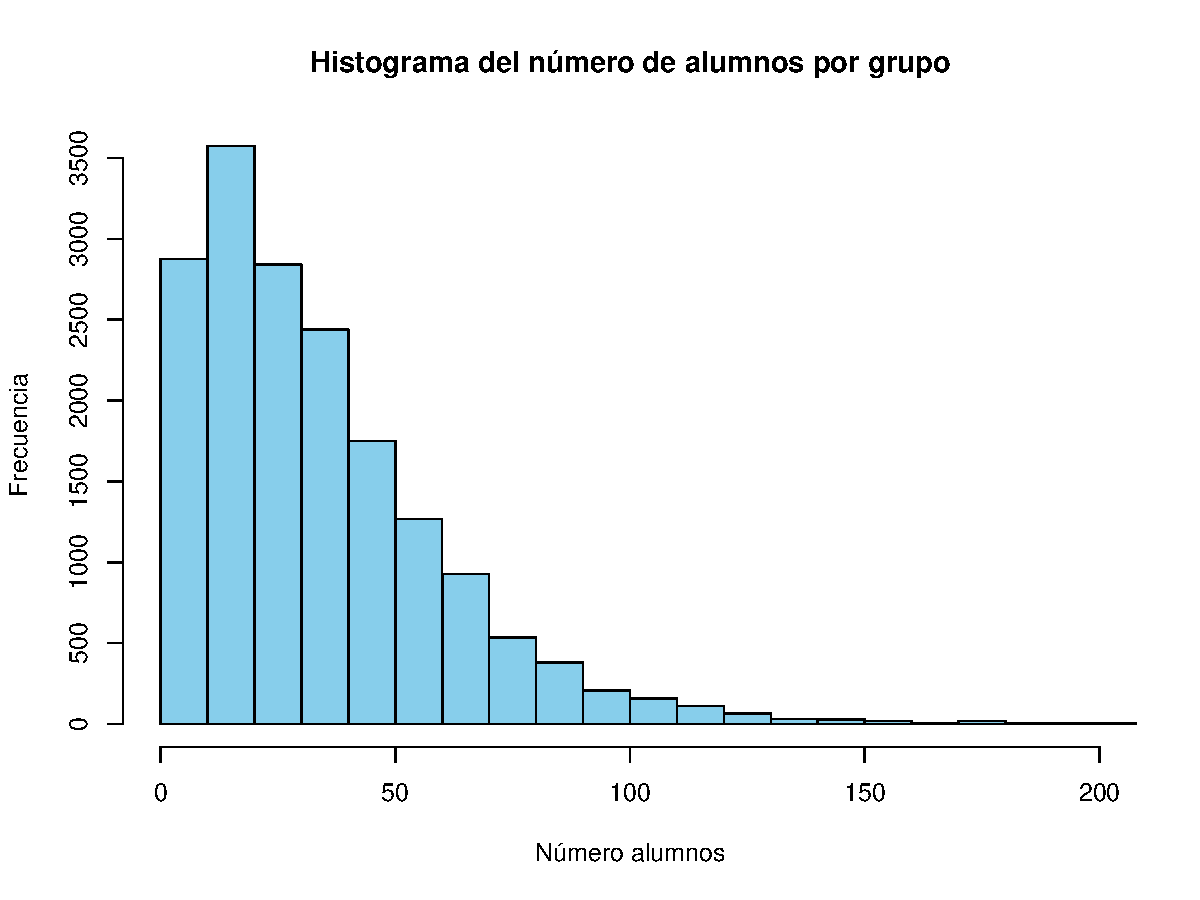
\includegraphics[scale = 0.8]{histograma_FA_num_alum_x_gpo_x_sem.pdf} %width=\textwidth
\caption{\textit{Histograma del número de alumnos por grupo de todos los semestres}}\label{histNumAl_x_gpo_x_sem}
\end{figure}


En la figura \ref{densidadesNumAl_x_gpo_x_sem} vemos diferentes líneas con las densidades ajustadas a los valores del número de alumnos por grupo de cada semestre. Cada línea corresponde a un semestre. Se tomaron los datos de 25 semestres, del 2008-1 al 2020-1. Notamos que el comportamiento es prácticamente el mismo en todos los semestres, salvo en dos cuyo pico máximo es mucho menor que los demás. 

\begin{figure}[H]
\centering
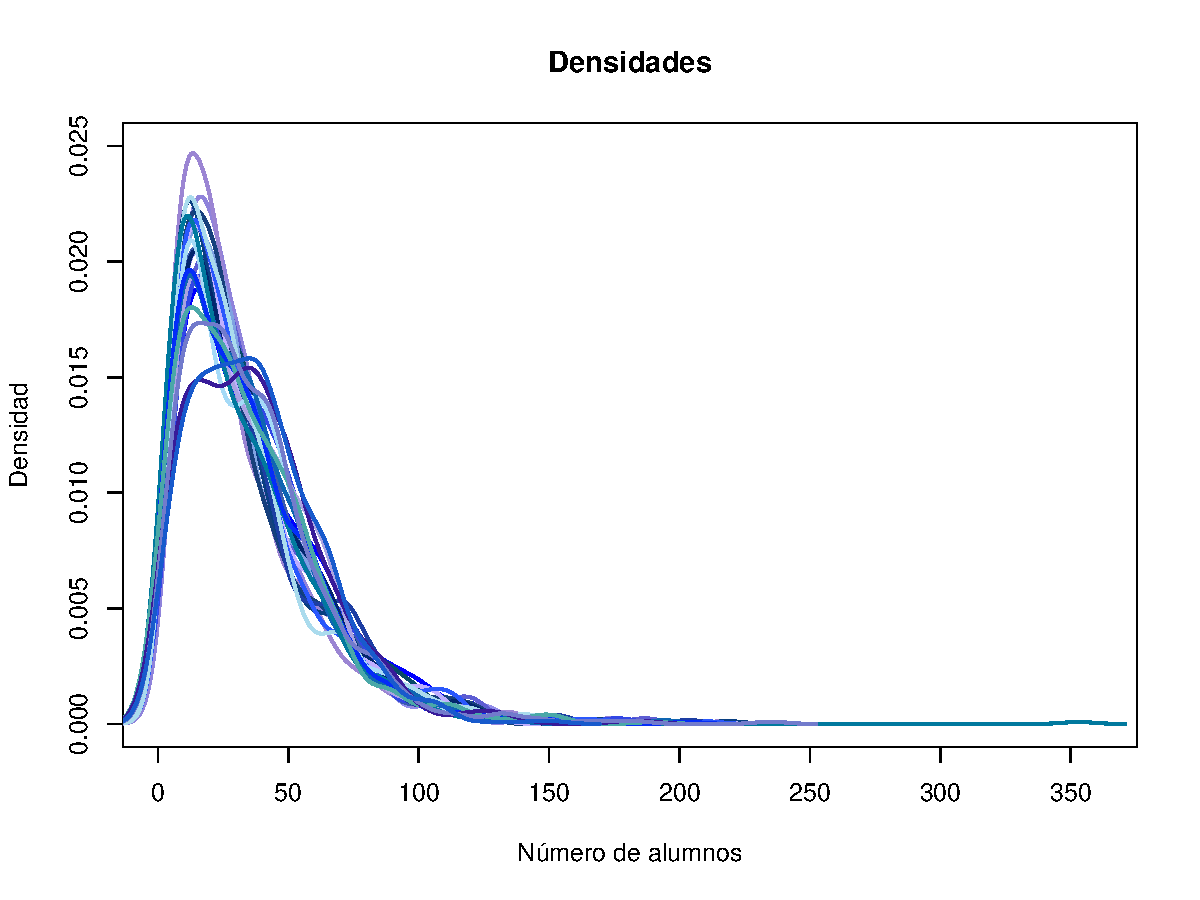
\includegraphics[scale = 0.8]{densidades_num_alum_x_gpo_x_sem.pdf} %width=\textwidth
\caption{\textit{Densidades del número de alumnos por grupo de cada semestre}}\label{densidadesNumAl_x_gpo_x_sem}
\end{figure}

Viendo las gráficas de las figuras \ref{histNumAl_x_gpo_x_sem} y \ref{densidadesNumAl_x_gpo_x_sem}, podríamos concluir que la distribución que mejor se ajusta al tamaño de los grupos es la distribución Poisson por la forma en la que están distribuidos los datos. Para probar esta hipótesis utilizamos la función \verb@ks.test(X,Y)@, de \textit{R}, para hacer la prueba de Kolmogorov-Smirnov.

La prueba de Kolmogorov-Smirnov, dice que se rechaza $H_{0}$ cuando $D_{n} > D_{n}^{1-\alpha}$. Donde $D_{n}^{1-\alpha}$ nos indica el valor en donde inicia la región de rechazo para un nivel de significancia de $\alpha$ y $n$ es el número de datos de la muestra. Tomamos como hipótesis nula $H_{0}: X$ y $Y$ tienen la misma distribución.

Definimos a $X$ como el vector con el número de alumnos por cada grupo del semestre 2008-1 al 2020-1. Definimos a $Y$ como un vector de números aleatorios de una distribución $Poisson(\lambda)$. Por el resultado \ref{EMVlambda} sabemos que el estimador máximo verosímil de $\lambda$ para la distribución $Poisson(\lambda)$ es la media de los datos. Con este estimador, $(\hat{\lambda} = 34.18746),$ obtuvimos los números aleatorios de $Y$. Tenemos que $Y \sim Poisson(34.18)$.

Por \ref{Miller} sabemos que:

\begin{equation}\label{Dn_KS}
D_{n}^{1-\alpha} = \sqrt{\dfrac{ln \left(\dfrac{1}{\alpha}\right)}{2n}} - 1.6693 n^{-1} - 0.20562 n^{-\frac{3}{2}}
\end{equation}

En nuestro caso los valores de las variables son: $n = 17,246$ y $\alpha = 0.01$. Sustituyendo en la ecuación \ref{Dn_KS} tenemos que $D_{17246}^{0.99} = 0.01145794823$. Con la función \verb@ks.test(X,Y)@, de \textit{R}, obtenemos el valor de $D_{17246} = 0.39974$

Como $D_{17246} = 0.39974 > 0.01145 = D_{17246}^{0.99} \Rightarrow $ se rechaza $H_{0}$, por lo tanto los datos no siguen una distribución Poisson con $\lambda = 34.18$.


Hicimos otra prueba suponiendo que los datos tienen una distribución $Normal(\mu,\sigma)$. Para simular los datos de $Y$ utilizamos los estimadores máximo verosímiles de $\mu$ y $\sigma$. Estos estimadores los obtuvimos con la función \verb@fitdistr(X, densfun="normal")@, en \textit{R}. Los valores de los estimadores son $\hat{\mu} = 34.1874638$ y $\hat{\sigma} = 26.5768345$. El resultado de la función de la prueba de Kolmogorov-Smirnov es $D_{17246} = 0.10513$.

Como $D_{17246} = 0.10513 > 0.01145 = D_{17246}^{0.99} \Rightarrow $ se rechaza $H_{0}$, por lo tanto los datos no siguen una distribución $Normal(34.18,26.57)$.

En la figura \ref{histFR_pruebaKS} vemos el histograma con las frecuencias relativas de los datos. La línea azul es la densidad ajustada generada por \textit{R}, la línea morada es la densidad de $n$ números aleatorios con distribución  $Poisson(34.18)$ y la línea roja es la densidad de $n$ números aleatorios con distribución  $Normal(34.18,26.57)$.

\begin{figure}[H]
\centering
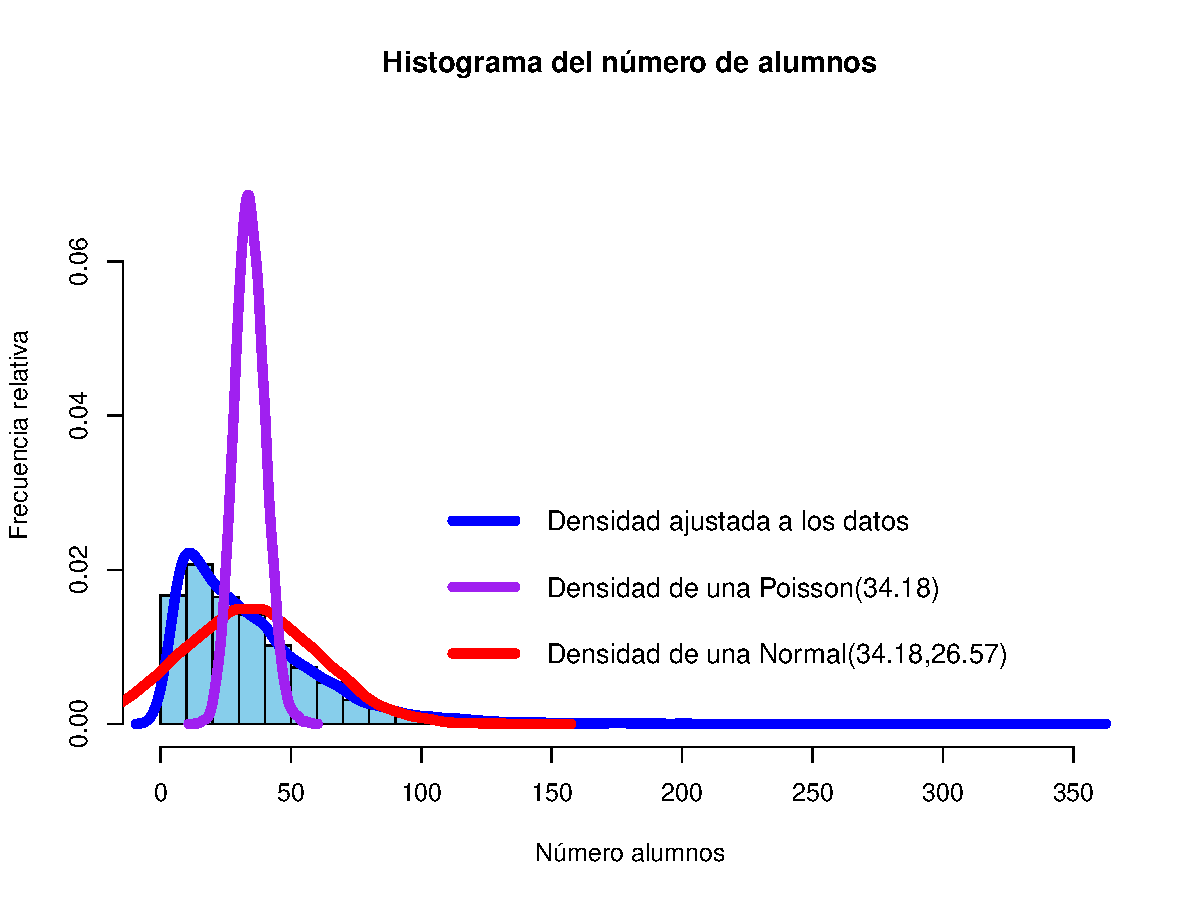
\includegraphics[scale = 0.8]{histograma_FR_prueba_KS.pdf} %width=\textwidth
\caption{\textit{Histograma con densidad ajustadad por prueba de Kolmogorov-Smirnov}}\label{histFR_pruebaKS}
\end{figure}

Hicimos más pruebas con otras distribuciones y en todos los casos rechazamos la hipótesis nula. Con estos resultados concluímos que el ajuste que se pudiera hacer a los datos tendría que ser en dos partes. Un ejemplo de una posible partición de los datos es que se puede ajustar una distribución para los datos que están entre 0 y 100, y otra distribución para los datos mayores a 100. Esto debido a que a pesar de ser pocos los datos mayores a 100, si impactan en la distribución total. El análisis con esta propuesta no lo realizamos para este trabajo.


\section{Comportamientos por hora}

En esta sección veremos algunas gráficas cuyo eje $x$ corresponde a las horas en las que se imparten las clases. Se empieza por la clase de 7-8hrs y se termina con la clase de 21-22hrs. Primero mostraremos el comportamiento del promedio de grupos por hora y después el comportamiento del promedio del número de alumnos por hora.

En la figura \ref{num_prom_gpos_x_hora_barplot} se muestra la gráfica de barras con el número promedio de grupos por hora. Se tomó la información de 25 semestres. Se observa una disminución considerable de los grupos a las 15hrs. Podemos concluir que es debido a que a esa hora, usualmente la gente sale a comer. A las 21hrs se tiene el menor número de grupos, esto se puede explicar por el hecho de que es la última clase impartida en la FC.

Hay un descenso leve a las 9hrs donde se pudiera suponer que la gente sale a desayunar. En mi caso particular, al estudiar la carrera de Actuaría, tenía clases desde las 7a.m. por lo que las 9a.m. era una buena hora para hacer una pequeña pausa en el horario y tener un descanso para desayunar. Esta hora coincide con el cambio en el que se dejan de impartir las materias exclusivas para los actuarios como Teoría del Seguro, MASP o MASD. Es decir, a partir de las 9 de la mañana se imparten materias de todas las carreras.

A las 10 de la mañana se tiene el número máximo de grupos. Con esta información se podría medir la capacidad que debería de tener la facultad en cuanto al número de salones necesarios para cubrir la demanda de grupos. Si se está preparado para cubrir la demanda del pico más alto de todas las horas, entonces los demás casos están cubiertos por tener menor número de grupos.


\begin{figure}[H]
\centering
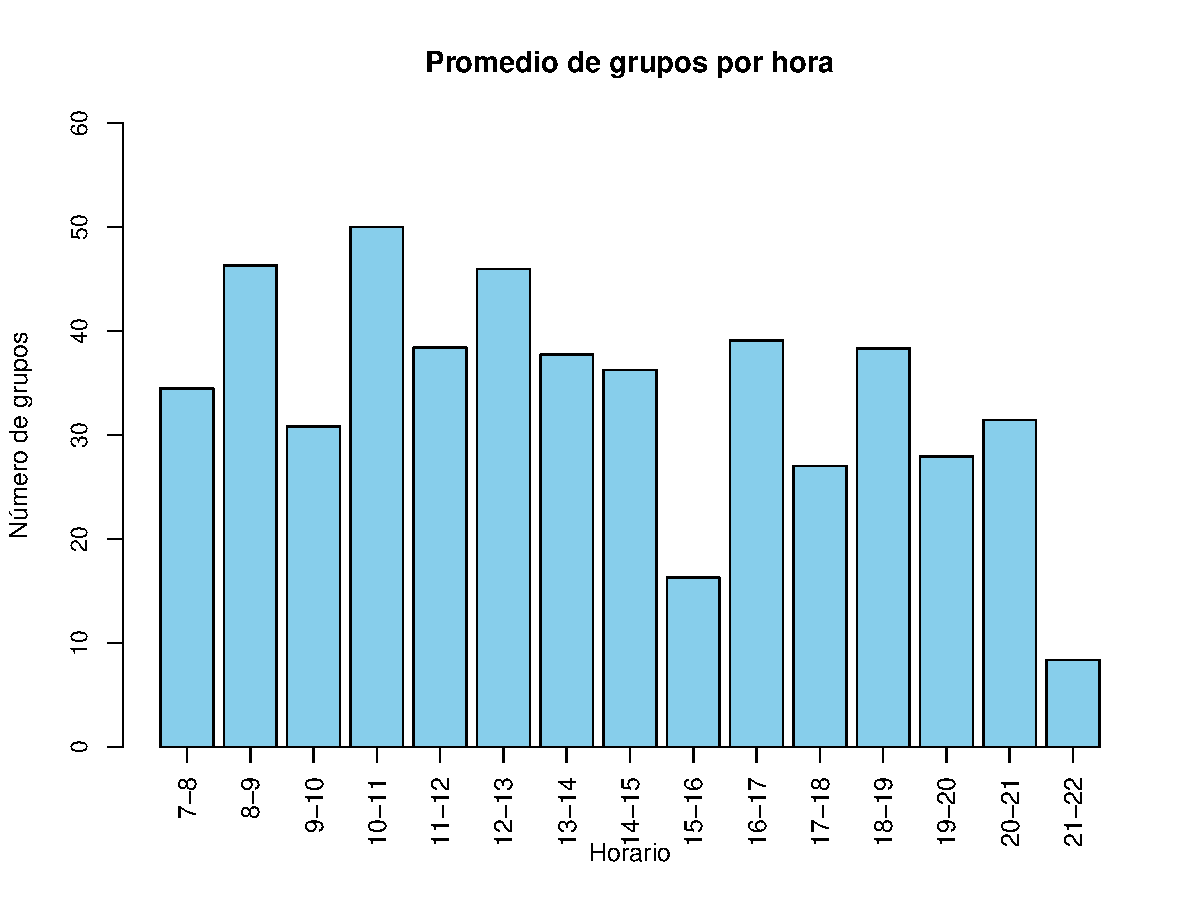
\includegraphics[scale = 0.8]{num_prom_gpos_x_hora_barplot.pdf} %width=\textwidth
\caption{\textit{Número promedio de grupos por hora}}\label{num_prom_gpos_x_hora_barplot}
\end{figure}

En la figura \ref{prom_alum_x_hora_barplot} se muestra la gráfica de barras con el promedio número de alumnos por hora. Notamos que el comportamiento de ésta gráfica es muy similar al de la gráfica mostrada en la figura \ref{num_prom_gpos_x_hora_barplot}. El pico más alto de los datos también se tiene a las 10 de la mañana y el menor número de alumnos se encuentra a las 21hrs. También hay una disminución considerable a las 15hrs. Esta correlación que existe entre ambos tipos de datos $\ldots$

\begin{figure}[H]
\centering
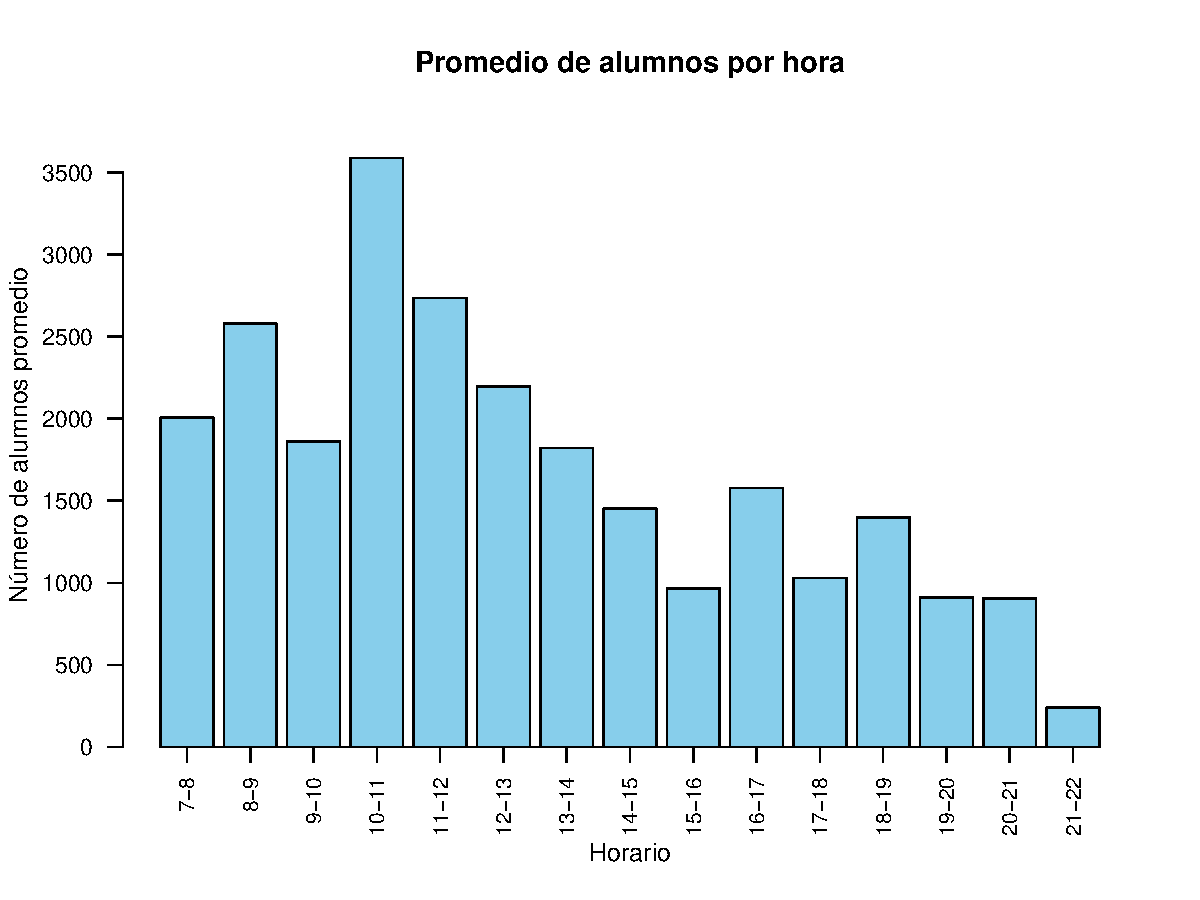
\includegraphics[scale = 0.8]{prom_alum_x_hora_barplot.pdf} %width=\textwidth
\caption{\textit{Número promedio de alumnos por hora}}\label{prom_alum_x_hora_barplot}
\end{figure}

